\documentclass{beamer}
\usepackage[serbian]{babel}
\usepackage[utf8]{inputenc}
\usepackage{tikz}
\usepackage{mathtools}
\usepackage{ragged2e}
\usepackage{caption}
\newtheorem{thm}{Theorem}[section] % the main one

% for specifying a name
\theoremstyle{plain} 
\newcommand{\thistheoremname}{}
\newtheorem{genericthm}[thm]{\thistheoremname}
\newenvironment{namedthm}[1]
  {\renewcommand{\thistheoremname}{#1}%
   \begin{genericthm}}
  {\end{genericthm}}


\definecolor{Boja}{RGB}{198,49,26}
\setbeamercolor{structure}{fg=Boja!90!black}

\beamertemplatenavigationsymbolsempty
\usetheme{Warsaw}

\setbeamertemplate{footline}
{
  \leavevmode%
  \hbox{%
  \begin{beamercolorbox}[wd=.4\paperwidth,ht=2.25ex,dp=1ex,center]{author in head/foot}%
    \usebeamerfont{author in head/foot}\insertshortauthor
  \end{beamercolorbox}%
  \begin{beamercolorbox}[wd=.6\paperwidth,ht=2.25ex,dp=1ex,center]{title in head/foot}%
    \hspace*{2em}\usebeamerfont{title in head/foot}\insertshorttitle\hspace*{3em}
  \end{beamercolorbox}}%
  \vskip0pt%
}

\title{Aproksimacija pravougaonika minimalnih površina i konveksnih kontejnera za pakovanje konveksnih poligona}
\subtitle{Geometrijski algoritmi - prezentacija rada iz časopisa}
\author[Nikola Belaković]{Nikola Belaković 1023/2023}
\institute[]{\\Matematički fakultet, Univerzitet u Beogradu}
\date[]{novembar 2023.}

\begin{document}
\begin{frame}
  \titlepage
\end{frame}

\begin{frame}\frametitle{Sadržaj}\tableofcontents
\end{frame} 

\section{O autorima, radu i problemu}
\subsection{Podaci o autorima}
\begin{frame}{O autorima}
    \begin{itemize}
        \item Journal of Computational Geometry 8(1) (2017) 1-10. 
        \item Autori rada su:
            \begin{itemize}  
                \item \textbf{Helmut Alt} (alt@mi.fu-berlin.de)\\
               Institute of Computer Science, Freie Universität Berlin, Germany\\
                \item \textbf{Mark de Berg} (mdberg@win.tue.nl)\\
                Department of Computing Science, Eindhoven, the Netherlands
                \item \textbf{Christian Knauer} (christian.knauer@uni-bayreuth.de)\\
                Universität Bayreuth, Institut für Angewandte Informatik, AG Algorithmen und Datenstrukturen (AI VI),Bayreuth, Germany     
            \end{itemize} 
    \end{itemize}
\end{frame}

\subsection{O problemu}
\begin{frame}{O problemu}
\begin{itemize}
    \item Klasičan problem kombinatorne optimizacije u geometriji
    \item Dat je skup konveksnih poligona $P$=\{$p{1}$,$p{2}$,...,$p{k}$\} sa ukupno $n$ tačaka 
    \item Problem pronalaženja kontejnera minimalne površine za razdvojeno pakovanje datog skupa konveksnih poligona pomoću translacije.
    \item Razmatraju se dva tipa kontejnera:
        \begin{itemize}
            \item Pravougaonik sa stranicama paralelnim osama
            \item Proizvoljni konveksni kontejner
        \end{itemize}
    \item Ovaj rad je prvi dokazao da se ovaj NP-teški optimizacioni problem uopšte može aproksimirati
        
\end{itemize}
\end{frame}

\subsection{Prethodna istraživanja}
\begin{frame}{Prethodna istraživanja varijanti ovog problema}
\begin{itemize}
        \item Najosnovniji problem je odlučivanje da li se dati skup objekata može upakovati u dati kontejner.
        \item Problemi kod kojih je oblik objekta pravougaonik rešivi sa faktorom optimizacije 2
        \item Problemi u kojima je dozvoljena rotacija
        \item Problemi pakovanja konveksnih poligona pod krutim pokretom rešivi sa faktorom optimizacije 4
        
\end{itemize}
\end{frame}

\subsection{Osnovni pojmovi}
\begin{frame}{Osvnovni pojmovi}
\begin{itemize}
    \item $h_{\text{max}} := \max_{p \in P} \text{height}(p)$ - najveća visina svih poligona
    \item $w_{\text{max}} := \max_{p \in P} \text{width}(p)$ - najveća širina svih poligona
    \item Skup poligona $P$ se deli u $visinske$ $klase$ pomoću parametra $\alpha$, $0<\alpha<1$, koji se određuje tako da faktor aproksimacije bude optimalan
    \item Kičma poligona $p$, u oznaci $s(p)$, predstavlja segment koji povezuje najnižu i najvišu tačku poligona $p$
    \item c - parametar koji se koristi za podelu mini-kontejnera i koji će biti određen tako da faktor aproksimacije bude optimalan
    
\end{itemize}
\end{frame}

\section{Pravougaoni kontejner}
\subsection{Algoritam}
\begin{frame}{Osnove algoritma}
\begin{itemize}
\item Skup $P$ se deli na skupove  tako da $P_i$ sadrži poligone $p\in P$ za koje važi $h_{i+1}<\text{height}(p)\leq h_i$, gde je $h_i=\alpha^i\cdot h_{max}$
    \item Opšta strategija algoritma se deli u dva koraka
    \begin{enumerate}
        \item Svaku visinsku klasu $P_i$ smestiti u kontejner $B_i$ visine $h_i$
        \item Svaki neprazan $B_i$ zameniti kolekcijom osno-poravnatih mini-kontejnera koji se smeštaju u kontejner $B$
    \end{enumerate}
    
    
\end{itemize}
\end{frame}

\subsubsection{Algoritam - korak 1}
\begin{frame}{Korak 1 - Pakovanje poligona iz jedne visinske klase}
\begin{itemize}
    \item Razmatramo visinsku klasu $P_i$ koja sadrži poligone čija visina leži u opsegu $(\alpha h_i, h_i]$
    \item Definišemo polustranicu $\sigma := [0, \infty) \times [0, h_i]$, polu-beskonačna pravougla traka visine $h_i$
    \captionsetup[figure]{justification=centering, , labelsep=colon, skip=4pt}
    \begin{figure}
        \centering
        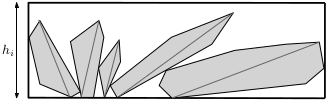
\includegraphics[width=0.8\textwidth]{slika1.png}
        \caption{Primer pakovanja skupa poligona iz jedne visinske klase}
    \end{figure}
    
    
\end{itemize}
\end{frame}

\begin{frame}{Korak 1 - Pakovanje poligona iz jedne visinske klase}
\begin{itemize}
    \item Poligone iz $P_i$ sortiramo prema nagibu njihovih kičmi i postavljamo ih u $\sigma$ sledeći pohlepni pristup
    \item Pomeramo ih što više na levo, sve dok ne udare u prethodno postavljeni poligon ili levi rub $\sigma$, zadržavajući najniži vrh na donjem rubu $\sigma$.
    \item Nakon što postavimo sve poligone, zatvaramo kontejner $B_i$, tako da desni rub $B_i$ određujemo vertikalnom linijom kroz najdesniji vrh bilo kog od postavljenih poligona.
    \begin{namedthm}{Lema 1.}
        Površina kontejnera $B_i$ za poligone $P_i$ zadovoljava formulu $\text{area}(B_i) \leq \frac{2}{\alpha} \cdot \sum_{p \in P_i} \text{area}(p) + 2h_i \cdot \max_{p \in P_i} \text{width}(p)$
    \end{namedthm}
\end{itemize}
\end{frame}


\subsubsection{Algoritam - korak 2}
\begin{frame}{Korak 2 - Generisanje i pakovanje mini-kontejnera}
\begin{itemize}
    \item Korak 1 rezultira kolekcijom kontejnera $B_i$ različitih dužina $l_i$
    \item Zamjenjujemo svaki $B_i$ mini-kontejnerima iste dužine na sledeći način:
      \begin{itemize}
        \item Delimo $B_i$ na kutije širine $c \cdot w_{\text{max}}$ i visine $h_i$, osim za poslednju kutiju koja može imati širinu manju od $w_{\text{max}}$.
        \item Svaki poligon $p \in P_i$ dodeljujemo kutiji koja sadrži njegov levi najviši vrh (ako levi najviši vrh leži na granici između dve kutije, dodeljujemo ga desnoj kutiji).
        \item Generišemo mini-kontejner iz svake kutije produžavajući je udesno dok joj širina ne postane tačno $(c + 1) \cdot w_{\text{max}}$.
      \end{itemize}
    \item Dobijamo kolekciju $R_i$ od najviše $l_i / (c \cdot w_{\text{max}}) + 1$ mini-kontejnera, svaki sa širinom tačno $(c + 1) \cdot w_{\text{max}}$.
    \begin{center}
        $\sum_{b \in R_i} \text{area}(b) \leq (1 +  \frac{1}{c}) \cdot \text{area}(B_i) + (c + 1)  w_{\text{max}} h_i$
    \end{center} 
\end{itemize}
\end{frame}

\subsection{Rezultati}
\begin{frame}{Rezultati}
\begin{itemize}
    \begin{namedthm}{Teorema 1.}
        Neka je $P$ skup poligona na ravni sa ukupno n temena. Možemo spakovati $P$ u vremenu $O(nlogn)$ u pravougaoni kontejner $B$ takav da je $\text{area}(B) \leq 17.45 \cdot opt$, gde je $opt$ minimalna površina bilo kog pravougaonog kontejnera za $P$
    \end{namedthm}
    \item Dokaz: Iz formule sa prošlog slajda, primenom Leme 1 dobija se da je $\text{area}(B) \leq ((1+\frac{1}{c})(\frac{2}{\alpha}+\frac{2}{1-\alpha})+\frac{c+1}{1-\alpha}) \cdot opt$
    \item Faktor ispred $opt$ se uprošćava na $f(c,\alpha) := (1+\frac{1}{c}) \cdot \frac{2+c\alpha}{\alpha-\alpha^2}$
    \item Korišćenjem parcijalnih izvoda za traženje optimalnih vrednosti za $\alpha$ i $c$ dobijamo da je $\alpha=0.407...,c=2.214...$ i $f(c,\alpha)=17.449...$
\end{itemize}
\end{frame}

\section{Konveksni kontejner}
\subsection{Algoritam}
\begin{frame}{Algoritam}
\begin{itemize}
    \item Tražimo $\varphi^* \in S^1$ koji minimizuje $h_{\text{max}}(\varphi)w_{\text{max}}(\varphi)$, gde je $h_{\text{max}}(\varphi)$ maksimalni opseg u pravcu koji je normalan na $\varphi$, a $w_{\text{max}}(\varphi)$ opseg u pravcu $\varphi$
    \item Pronalazimo $B$ kao u prethodnom algoritmu sa orijentacijom $\varphi^*$ i vraćamo ga kao rezultat algoritma
    \item Funkcije $h_{\text{max}}(\varphi)$ i $w_{\text{max}}(\varphi)$ sa sastavljene od funkcija $\alpha \cdot \sin{(\varphi+b)}$, za neke konstante $a, b \in \mathbb{R}$
    \item Broj ovih funkcija je jednak broju parova antipodalnih čvorova u svim poligonima
\end{itemize}
\end{frame}

\subsection{Rezultati}
\begin{frame}{Rezultati}
\begin{itemize}
    \begin{namedthm}{Teorema 2.}
        Neka je $P$ skup konveksnih poligona na ravni sa ukupno n temena. Možemo spakovati $P$ u vremenu $O(nlogn)$ u konveksni poligon $B$ takav da je $\text{area}(B) \leq 27 \cdot opt$, gde je $opt$ minimalna površina bilo kog pravougaonog kontejnera za $P$
    \end{namedthm}
    \item Dokaz: Kao za Teoremu 1. sa korišćenjem dodatne formule $h_{\text{max}}(\varphi^*) \cdot w_{\text{max}}(\varphi^*) \leq h_{\text{opt}} \cdot w_{\text{opt}} = \text{area}(B_{\text{opt}}) \leq 2 \cdot \text{opt}$
    \item Dobija se da je $\text{area}(B) \leq \frac{c+1}{c}(\frac{2}{\alpha}+\frac{4}{1-\alpha}+\frac{2c}{1-\alpha}) \cdot opt$
    \item Faktor ispred $opt$ će biti $f(c,\alpha) := \frac{c+1}{c}(\frac{2}{\alpha}+\frac{4}{1-\alpha}+\frac{2c}{1-\alpha})$
    \item Korišćenjem parcijalnih izvoda za traženje optimalnih vrednosti za $\alpha$ i $c$ dobijamo da je $\alpha=1/3,c=2$ i $f(c,\alpha)=27$
\end{itemize}
\end{frame}


\section{Primena i zaključak}
\begin{frame}{Primena i zaključak}
\begin{itemize}
    \item Primena ovih algoritama je velika i značajna
    \begin{enumerate}
        \item Obrada lima i odeće - isecanje skupa uzoraka iz velikog komada materijala minimizirajući otpad
        \item Problem pakovanja trake - skup objekata je potrebno upakovati na traku određene fiksne širine koristeći što kraći deo trake
        \item Minimiziranje skladišnih kontejnera - u tri dimenzije
    \end{enumerate}
    \item Rezultati pokazuju da se ovaj NP-teški optimizacioni problem može aproksimirati
    \item Faktor aproksimacije je veliki, ali trenutno ne postoji bolji rezultat od ovog
    \item U budućnosti treba uraditi iste stvari samo da umesto translacije bude dozvoljena i rotacija poligona
\end{itemize}
\end{frame}

\section{Literatura}
\begin{frame}{Literatura}
\begin{itemize}
    \item A. Steinberg. A strip-packing algorithm with absolute performance bound 2. SIAM J. Comput., 26(2):401 409, Apr. 1997.
    \item R. Harren, K. Jansen, L. Pradel, and R. van Stee. A (5/3 + e)-approximation for strip packing. Comput. Geom., 47(2):248 267, 2014.
    \item L. von Niederhausern. Packing polygons. Master's thesis, EPFL Lausanne, FU Berlin, 2014.
    \item H.-K. Ahn and O. Cheong. Aligning two convex figures to minimize area or perimeter. Algorithmica, 62(1-2):464 479, 2012.
\end{itemize}
\end{frame}
\end{document}